\documentclass[a4paper,11pt]{article}
\usepackage[utf8]{inputenc}
\usepackage{lastpage}
\usepackage{fancyhdr}
\usepackage[english]{babel}
\usepackage[a4paper,margin=1in]{geometry}
\usepackage{multirow}
\usepackage[table,xcdraw]{xcolor}
\usepackage{array}
\usepackage{amsmath}
\usepackage{amssymb}
\usepackage{relsize}
\usepackage{algorithm}
\usepackage{algpseudocode}
\usepackage{graphicx}
\usepackage[numbered,framed]{matlab-prettifier}


\newcolumntype{L}[1]{>{\raggedright\let\newline\\\arraybackslash\hspace{0pt}}m{#1}}
\newcolumntype{C}[1]{>{\centering\let\newline\\\arraybackslash\hspace{0pt}}m{#1}}
\newcolumntype{R}[1]{>{\raggedleft\let\newline\\\arraybackslash\hspace{0pt}}m{#1}}

\def\margin#1#2{\list{}{\rightmargin#2\leftmargin#1}\item[]}
\let\endmargin=\endlist

\newcommand\tab[1][4mm]{\hspace*{#1}}
\newcommand{\norm}[1]{\left\lVert \mathbf{#1} \right\rVert}
\newcommand{\abs}[1]{\left\vert #1 \right\vert}

%-------------------------------------------------------------------------------
% HEADER & FOOTER
%-------------------------------------------------------------------------------

\pagestyle{fancy}
\fancyhf{}
\setlength\headheight{15pt}
\fancyhead[L]{ Numerical Analysis Assignment 1 }
\fancyhead[R]{Student ID: 100633486}
\fancyfoot[R]{Page \thepage\ of \pageref{LastPage}}


%-------------------------------------------------------------------------------
% TITLE PAGE
%-------------------------------------------------------------------------------

\begin{document}

\title{
	\Huge \textbf {Numerical Analysis}
    \\ [0.2cm]
	\LARGE Assignment 1, October 2017
    \\ [0.5cm]
    \hrule
}

\date{}

\author{
		\Large Kamyar Nazeri \\
		\large Student ID: 100633486 }

\maketitle

\newpage

\section*{Question 1.}
(a) Provide an example of a $3 \times 3$ skew-symmetric matrix.
\begin{align*}
B = \begin{bmatrix}
       0 & 1 & 2 \\
       -1 & 0 & 3 \\
       -2 & -3 & 0
     \end{bmatrix}
\end{align*}
\\
(b) Let $A=(I+B)(I-B)^{-1}$ and show that $A^{-1}=A^{T}$ if $B$ is skew-symmetric.
\\
\begin{margin}{0.5cm}{0.5cm}
We know
\begin{align*}
B^{T}\ =\ -B
\end{align*}
We need to show $A^{T}A=I$ and conclude $A^{-1}=A^{T}$ \\
\begin{align}
\begin{split}
A^{T}A
&=\bigg((I+B)(I-B)^{-1}\bigg)^{T}\bigg((I+B)(I-B)^{-1}\bigg)\\
&=\bigg(\bigg[(I-B)^{-1}\bigg]^{T}(I+B)^{T}\bigg)\bigg((I+B)(I-B)^{-1}\bigg)\\
&=\bigg(\bigg[(I-B)^{T}\bigg]^{-1}(I+B)^{T}\bigg)\bigg((I+B)(I-B)^{-1}\bigg) \\
&=\bigg((I-B^{T})^{-1}(I+B^{T})\bigg)\bigg((I+B)(I-B)^{-1}\bigg) \\
&=\bigg((I+B)^{-1}(I-B)\bigg)\bigg((I+B)(I-B)^{-1}\bigg) \\
&=(I+B)^{-1}\bigg((I-B)(I+B)\bigg)(I-B)^{-1}
\end{split}
\end{align}
\\
We know for every square matrix $B$:
\begin{align}
(I-B)(I+B) = (I+B)(I-B)
\end{align}
Equation (1) becomes:
\begin{align}
\begin{split}
A^{T}A
&=(I+B)^{-1}\bigg((I+B)(I-B)\bigg)(I-B)^{-1} \\
&=\bigg((I+B)^{-1}(I+B)\bigg)\bigg((I-B)(I-B)^{-1}\bigg) \\\\
&= (I)(I) \\\\
&= I
\end{split}
\end{align}
\end{margin}

\newpage

\section*{Question 2.}
Assume that \textbf{x} is a vector in $C^{n\times1}$. Prove the following inequality and provide example of a vector for which equality is achieved. $\frac{1}{n}\norm{x}_1\leq\norm{x}_{\infty}\leq\norm{x}_2$ \\
\begin{margin}{0.5cm}{0.5cm}
let $\mathbf{x}=\{x_1,x_2,x_3,...,x_n\}$ \\\\
\noindent\rule{8cm}{0.4pt} \\
$
x_1 + x_2 + ... + x_n \leq \max\limits_{\mathsmaller{1\leq k\leq n}} \abs{x_k} + \max\limits_{\mathsmaller{1\leq k\leq n}} \abs{x_k} + ... + \max\limits_{\mathsmaller{1\leq k\leq n}} \abs{x_k} \\
\sum\limits_{k=1}^{n}\abs{x_k} \leq n\big(\max\limits_{\mathsmaller{1\leq k\leq n}} \abs{x_k}\big) \\
\frac{1}{n}\big(\sum\limits_{k=1}^{n}\abs{x_k}\big) \leq \max\limits_{\mathsmaller{1\leq k\leq n}} \abs{x_k} \\\\
\frac{1}{n}\norm{x}_1\leq\norm{x}_{\infty}
$
\\
\noindent\rule{8cm}{0.4pt} \\
$
\max\limits_{\mathsmaller{1\leq k\leq n}} \abs{x_k} \leq \bigg(\abs{x_1}^{2}+\abs{x_2}^{2}+...+\max\limits_{\mathsmaller{1\leq k\leq n}} \abs{x_k}^{2}+...+\abs{x_n}^{2} \bigg)^\frac{1}{2} \\
\max\limits_{\mathsmaller{1\leq k\leq n}} \abs{x_k} \leq \sqrt{\sum\limits_{k=1}^{n}\abs{x_k}^{2}} \\\\
\norm{x}_{\infty}\leq\norm{x}_2
$
\\
\noindent\rule{8cm}{0.4pt} \\
\\
eg. $\mathbf{x}=\{1,2,3,...,x_n\} \tab\tab \frac{1}{n}\norm{x}_1\leq\norm{x}_{\infty}\tab\equiv\tab \frac{1}{n}\frac{n(n+1)}{2}\leq n $ \\
eg. $\mathbf{x}=\{1,2,3, 4\} \tab\tab\tab\tab \norm{x}_{\infty}\leq\norm{x}_{2}\tab\ \equiv\tab 4\leq \sqrt{30} $ \\
eg. $\mathbf{x}=\{1,1,1,...,1\} \tab\tab \frac{1}{n}\norm{x}_1\leq\norm{x}_{\infty}\leq\norm{x}_{2}\tab\equiv\tab \frac{1}{n}n\leq 1 \leq \sqrt{n} $ \\
\end{margin}

\section*{Question 3.}
Let $A \in \mathbb{C}^{n\times n}$ be a nonsingular matrix.\\
(a) Given $\mathbf{u}, \mathbf{v} \in \mathbb{C}^{n\times 1}$, prove that
\begin{align}
\setcounter{equation}{0}
\big[A-\mathbf{u}\mathbf{v}^H\big]^{-1}=A^{-1}+\frac{A^{-1}\mathbf{u}\mathbf{v}^HA^{-1}}{1-\mathbf{v}^HA^{-1}\mathbf{u}}
\end{align}

\begin{margin}{0.5cm}{0.5cm}
Multiply both sides by $(A-\mathbf{u}\mathbf{v}^H)$:\\\\
$
I=\bigg(A-\mathbf{u}\mathbf{v}^H\bigg)\bigg(A^{-1}+\frac{A^{-1}\mathbf{u}\mathbf{v}^HA^{-1}}{1-\mathbf{v}^HA^{-1}\mathbf{u}}\bigg) \\
I=\bigg((A-\mathbf{u}\mathbf{v}^H)A^{-1}\bigg)+\bigg(\frac{(A-\mathbf{u}\mathbf{v}^H)(A^{-1}\mathbf{u}\mathbf{v}^HA^{-1})}{1-\mathbf{v}^HA^{-1}\mathbf{u}}\bigg) \\
I=\bigg(I-\mathbf{u}\mathbf{v}^HA^{-1}\bigg)+\bigg(\frac{AA^{-1}\mathbf{u}\mathbf{v}^HA^{-1}-\mathbf{u}\mathbf{v}^HA^{-1}\mathbf{u}\mathbf{v}^HA^{-1}}{1-\mathbf{v}^HA^{-1}\mathbf{u}}\bigg) \\
I=\bigg(I-\mathbf{u}\mathbf{v}^HA^{-1}\bigg)+\bigg(\frac{\mathbf{u}\big(1-\mathbf{v}^HA^{-1}\mathbf{u}\big)\mathbf{v}^HA^{-1}}{1-\mathbf{v}^HA^{-1}\mathbf{u}}\bigg) \tab\tab\tab\tab\tab\tab\tab\tab\tab \big(1-\mathbf{v}^HA^{-1}\mathbf{u}\big) $ is scaler$ \\
I=\bigg(I-\mathbf{u}\mathbf{v}^HA^{-1}\bigg)+\bigg(\mathbf{u}\mathbf{v}^HA^{-1}\bigg) \\\\
I=I
$
\end{margin}
\newpage
\noindent
(b) Based on the Sherman-Morrison formula (1), write an algorithm (in pseudocode) to explain how you would compute the solution $x \in \mathbb{C}^n$ of the system of equations \\\\
\begin{align}
\setcounter{equation}{0}
(A-\mathbf{u}\mathbf{v}^H)\mathbf{x}=\mathbf{b}
\end{align}
\begin{align}
\big[A-\mathbf{u}\mathbf{v}^H\big]^{-1}=A^{-1}+\frac{A^{-1}\mathbf{u}\mathbf{v}^HA^{-1}}{1-\mathbf{v}^HA^{-1}\mathbf{u}}
\end{align}

\begin{algorithm}
\caption{Solve a system of equations using Sherman-Morrison formula}\label{euclid}
    \begin{algorithmic}[1]
        \Procedure{Solve}{$A,u,v,b$}\Comment{input matrix $\mathbf{A}$ and vectors $\mathbf{u}$, $\mathbf{v}^H$ and $\mathbf{b}$}
        \State $ai\gets \textbf{inv}(A)$ \Comment{$A^{-1}$: $n^2$ flops}
        \State $aiu\gets \textbf{Ainv}(u)$ \Comment{$A^{-1}\mathbf{u}$: $n^2$ flops}
        \State $vai\gets v\times ai$ \Comment{$\mathbf{v}^{H}A^{-1}$: $2n^2$ flops}
        \State $numerator\gets aiu\times vai$ \Comment{$A^{-1}\mathbf{u}\mathbf{v}^{H}A^{-1}$: $n^2$ flops}
        \State $denominator\gets 1 - v \times aiu$ \Comment{$1-\mathbf{v}^{H}A^{-1}\mathbf{u}$: $2n$ flops}
        \State $result\gets ai - numerator \div denominator$ \Comment{$2n^2$ flops}
        \State $x\gets result \times b$ \Comment{$2n^2$ flops}
        \State \textbf{return} $x$
        \EndProcedure
    \end{algorithmic}
\end{algorithm}
\noindent
There are $(9n^2+2n)$ flops in this algorithm, which makes the complexity $O(n^2)$ 

\section*{Question 4.}
Which among the following approximations of $\pi$ better limits the propagation of rounding errors?

\begin{align}
\setcounter{equation}{0}
\pi = 4 \times \bigg(1 - \frac{1}{3} + \frac{1}{5} - \frac{1}{7} + \frac{1}{9}-...\bigg)
\end{align}

\begin{align}
\pi = 6 \times \bigg(0.5 + \frac{(0.5)^3}{2\times3} + \frac{3\times(0.5)^5}{2\times4\times5}+\frac{3\times5\times(0.5)^7}{2\times4\times6\times7}+...\bigg)
\end{align}
\\
\begin{margin}{0.5cm}{0.5cm}
The second series (2) better limits the rounding error. As demonstrated in the following table, by summing 23 items in the second series the error hits the minimum rounding error defined for double precision IEEE floating-point; $4.4409e-16 \simeq 2^{-53}$, while the first (1) series is still oscillating around $\pi$:
\end{margin}

\begin{center}
\begin{table}[h!]
\small
\begin{tabular}{ |c|c|c|c|c|c|c|c|c|c| }
 \hline
 n & 1 & 2 & 5 & 10 & 23 & 50 & 100 & 1000 \\
 \hline
 (1) error & 0.8584 & 0.4749 & 0.1981 & 0.0998 & 0.0435 & 0.0200 & 0.0100 & 1.0000e-03 \\
 \hline
 (2) error & 0.1416 & 0.0166 & 8.1481e-05 & 3.0719e-08 & 4.4409e-16 & 4.4409e-16 & 4.4409e-16 & 4.4409e-16 \\
 \hline
\end{tabular}
\caption{Absolute errors using first (n) items of the series to approximate $\pi$}
\end{table}
\end{center}

\newpage
\noindent
The following figure (\emph{figure 1}) demonstrates the approximation value and its absolute error as a function of number of terms in the series: 
\begin{figure}[!htb]
  \centering
  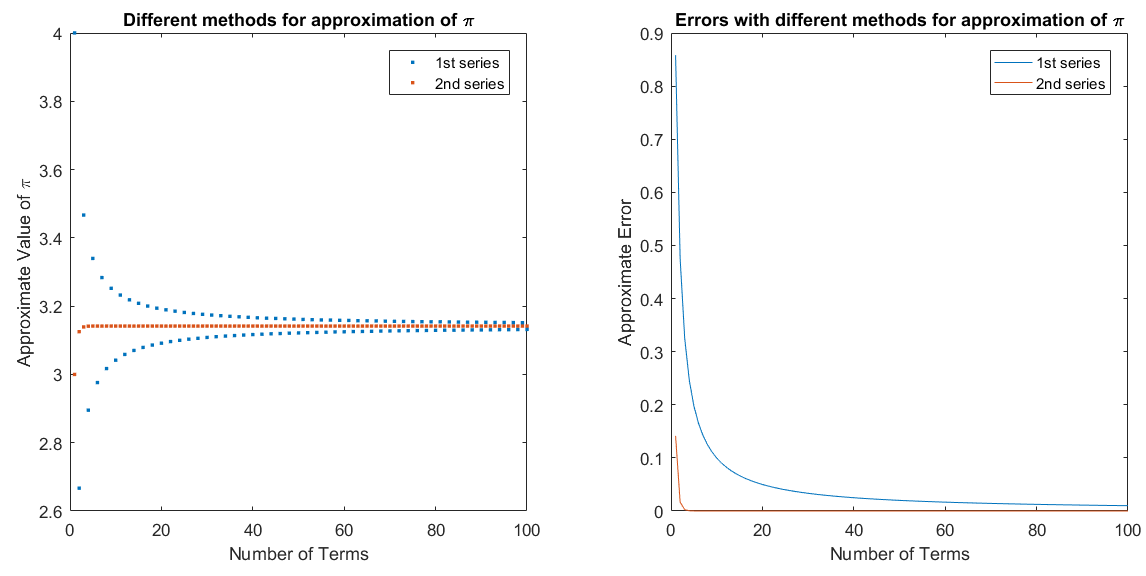
\includegraphics[width=16cm, height=8cm]{plots.png}
  \caption{\small Left: approximation of $\pi$ as a function of number of terms. Right: absolute error of the approximation as as a function of number of terms.}
\end{figure}

\noindent
\\The following Matlab function, calculates the first (1) series, taking argument (n) the number of the terms in the sum.
\begin{lstlisting}[
    style=Matlab-editor,
    numbers=none,
    frame=none,
    xleftmargin=.2in
]
function res = Pi1(n)
    res = 0;
    for i=1:n
        res = res + (-1)^(i+1) * 4 / (2*i-1);
    end
end
\end{lstlisting}

\noindent
\\\\The following Matlab function, calculates the second (2) series, taking argument (n) the number of the terms in the sum.
\begin{lstlisting}[
    style=Matlab-editor,
    numbers=none,
    frame=none,
    xleftmargin=.2in
]
function res = Pi2(n)
    res = 0;
    c = 1;
    for i=1:n
        p = (2*i - 1);
        res = res + (6 * c * 0.5^p / p);
        c = c * (p / (2*i));
    end
end
\end{lstlisting}

\newpage
\section*{Question 5.}
\setcounter{equation}{0}
Let $x, y, \tilde{x}, \tilde{y} \in \mathbb{C}$ be nonzero scalars. Show that
\begin{align}
\abs{\frac{xy-\tilde{x}\tilde{y}}{xy}}\leq(2+\epsilon)\epsilon \tab\tab\tab where \tab \epsilon:=\max\bigg\{\frac{\abs{x-\tilde{x}}}{\abs{x}},\frac{\abs{y-\tilde{y}}}{\abs{y}}\bigg\}
\end{align}
\\
\begin{margin}{0.5cm}{0.5cm}
    The absolute error in computing $xy$ is:
    \begin{align*}
        \abs{xy-\tilde{x}\tilde{y}}
        &= \abs{xy-\tilde{x}\tilde{y}+ \tilde{x}y - \tilde{x}y} \leq \abs{xy-\tilde{x}y}+\abs{\tilde{x}y-\tilde{x}\tilde{y}} \\
        &\leq \abs{xy}(\frac{\abs{x-\tilde{x}}}{\abs{x}})+\abs{\tilde{x}y}(\frac{\abs{y-\tilde{y}}}{\abs{y}}) \leq \abs{xy}\epsilon+\abs{\tilde{x}y}\epsilon \\
        &= \abs{xy}\epsilon+\abs{\tilde{x}y}\epsilon + \abs{xy}\epsilon - \abs{xy}\epsilon = \abs{xy}(\frac{\abs{x-\tilde{x}}}{\abs{x}})\epsilon + 2\abs{xy}\epsilon \\
        &\leq \abs{xy}\epsilon^2+\abs{xy}\epsilon
    \end{align*}
    And relative condition number of multiplication becomes:
    \begin{align*}
    \frac{\abs{xy-\tilde{x}\tilde{y}}}{\abs{xy}} \leq \frac{\abs{xy}\epsilon^2+2\abs{xy}\epsilon}{\abs{xy}} = (2+\epsilon)\epsilon
    \end{align*}
    \\\\
    If $\epsilon\leq1 \tab\Rightarrow\tab \epsilon^2 \leq \epsilon \tab\Rightarrow\tab 2\epsilon+\epsilon^2 \leq 2\epsilon+\epsilon=3\epsilon\tab$ and \\
    \begin{align*}
    \frac{\abs{xy-\tilde{x}\tilde{y}}}{\abs{xy}} \leq 3\epsilon
    \end{align*}
\end{margin}

\end{document}
